\subsection{Radar Simulations} \label{compvis_radarsims}

    \subsubsection{Introduction and Physical Principles} \label{rory_radar_principles}
    
        \noindent As described in Section \ref{simulation_justification}, the limited diversity of the radar dataset necessitates physics-driven simulations to replicate the noise and clutter encountered in real-world environments. The simulations in this section aim to test the radar model's robustness to the physical processes not represented in the training data, that degrade B-can clarity: scattering, attenuation, antenna and transmission losses.
        
        \noindent To model these effects, finite-difference time-domain (FDTD) simulations were conducted using \textit{gprMax} \cite{warren2016gprmax}, an open-source framework for solving Maxwell’s equations in 3D. These simulations capture full-wave electromagnetic behaviour, including wave propagation, reflection, and attenuation, and explicitly account for soil heterogeneity. Surface roughness is not considered in this section, but for the purposes of validating the models robustness it is not required. This is however a significant contribution to the clutter in an actual B-scan, and future work should consider this aspect.
     
    
    \subsubsection{gprMax Implementation}

        \paragraph{Radar}
        
             \noindent The radar configuration follows recommendations by Huirui (Section \ref{hardware}), and a Ricker waveform is used as the excitation signal. A central frequency of 1.5\,GHz was used, as it provides a good compromise between penetration depth and resolution, as shown in Section \ref{hardware}. The transmitter and receiver are modelled as Herzian dipole antennas \footnote{\url{https://engineering.purdue.edu/wcchew/ece604s21/Lecture\%20Notes/Lect25.pdf}} 10cm from the surface of the soil, and separated from each other by 2cm. B-scans are produced by taking successive A-scans while moving the source and receiver in 4\,mm increments from left to right across the simulation domain
    
        \paragraph{Domain}

            \noindent The simulated computational domain spans $0.8\times 0.3\times0.02$\,m ($x\times y\times z$), representing a quasi-2D space. The domain is discretised into cubic elements of side length 0.002\,m , 100 times smaller than the wavelength of the radar pulse\footnote{The wavelength of the pulse at the central frequency is 20~cm}. Two thirds of the domain is occupied with soil, and the rest with air. A circular landmine with radius 5\,cm is buried with its centre 0.1\,m below the surface of the soil, and is modelled as a perfect electric conductor (PEC), representative of a metallic landmine. See Figure \ref{fig:radar_domain} for a visualisation of the simulation domain.


        \paragraph{Boundary Conditions}
        
            \noindent Perfectly matched layers (PMLs) \footnote{\url{https://en.wikipedia.org/wiki/Perfectly_matched_layer}} are used as absorbing boundary conditions on all sides of the domain, to mimic an open boundary. The source and receiver were placed more than 20 cells away from the PML regions to avoid erroneous interference, as is advised in the gprMax docs. Each simulation was run for 5$\times$10$^{\text{-9}}$\,s, enough to capture all the relevant electromagnetic phenomena.
            \begin{figure}[htbp]
            \centering
            \begin{minipage}[b]{0.48\textwidth}
                \centering
                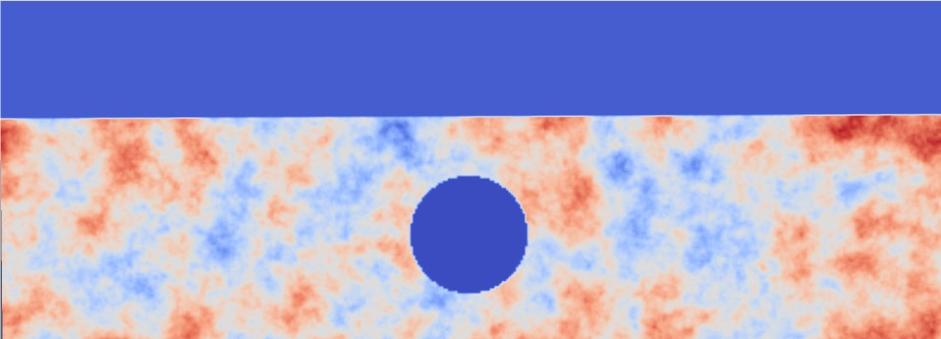
\includegraphics[width=\textwidth]{figs/Rory/radar_domain.pdf}
                \caption[Simulation domain]{Simulation domain viewed in ParaView \tablefootnote{\url{https://www.paraview.org/}}}
                \label{fig:radar_domain}
            \end{minipage}
            \hfill
            \begin{minipage}[b]{0.48\textwidth}
                \centering
                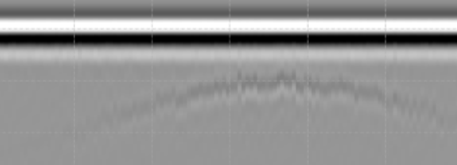
\includegraphics[width=\textwidth]{figs/Rory/sim_bscan_cropped.png}
                \caption{Raw simulated B-scan (no digital enhancement)}
                \label{fig:original_bscan}
            \end{minipage}
        \end{figure}    
    \subsubsection{Heterogeneous Soil Model}
    
        \noindent The heterogeneous soil is modelled using the Peplinski model, detailed in \cite{warren2016gprmax}. The model characterises soil dielectric properties based on sand fraction, clay fraction, bulk density, sand-particle density and volumetric water fraction range. To capture natural spatial variability, a fractal generation technique is employed, where self-similar patterns observed in natural soils are replicated over multiple scales (also detailed in Warren et al.).

        \paragraph{Soil Parameters}

            For the simulation to give physically realistic results, it is initialised with accurate soil data for Ukraine. Ukraine is mostly covered with the very fertile Chernozem soil \footnote{\url{https://www.britannica.com/place/Ukraine/Soils}}, the properties of which were taken from \cite{suleymanov2021chernozem}, and are summarised here in Table \ref{tab:chernozem}.

            \begin{table}[htbp]
              \centering
              \caption{Properties of Chernozem Soils}
              \begin{tabular}{@{} l l @{}} 
                \toprule
                \textbf{Property} & \textbf{Value} \\
                \midrule
                Clay fraction & $\sim 30\%$ \\
                Sand fraction & $\sim 70\%$ \\
                Bulk density & $\sim 1.4$ g/cm$^3$ \\
                Sand particle density & $2.65$ g/cm$^3$ \\
                Volumetric water fraction range & $1\% - 10\%$ \\
                \bottomrule
              \end{tabular}
              \label{tab:chernozem}
            \end{table}
    

    
    \subsubsection{Simulation Results and Validation}

        \noindent Figure~\ref{fig:original_bscan} shows the simulated noisy radar B-scan. Approximately 100 images like this are required to test the radar YOLO model without bias. A comparison with the 'clean' B-scans in the training set (Section \ref{computervision}) shows that the simulated B-scan also has a faint parabola indicating the landmine, and a bold line representing the reflection from the soil surface, and thus the simulations are somewhat validated with other data. However, the simulation assumes a simplified environment with flat ground, an absence of foliage, and the absence of puddles or other surface irregularities. These factors may account for discrepancies between simulated and real-world data.

    
    \subsubsection{Data Augmentation}

      Running these simulations is computationally intensive (\(\approx\) 30 minutes per simulation), so the most should be made of each simulation. From one simulation, multiple image augmentations were applied, each representing a physical process. The transforms considered were stretching (representing different soil properties and mine shape), cropping (representing B-scans that did not capture the whole mine), adding Gaussian blur (representing greater attenuation of high frequencies due to different soil properties), and combinations of these. Contrast limited adaptive histogram equalisation (CLAHE) \footnote{\url{https://en.wikipedia.org/wiki/Adaptive_histogram_equalization}} is also applied to every transformed image, to enhance image clarity whilst keeping the contrast manageable. When these transformations were applied to the simulated B-scan, a dataset of 90 images was generated, 3 of which are shown in Figure \ref{fig:sim_bscan_comparison} with the bounding box predictions from the pre-trained YOLO model. This is sufficient to test whether the pre-trained CNN (Section \ref{compvis_implementation}) is robust to heterogeneous soil properties and other physical loss phenomena.

        
        \begin{figure}[htbp]
          \centering
        
          \adjustbox{valign=c}{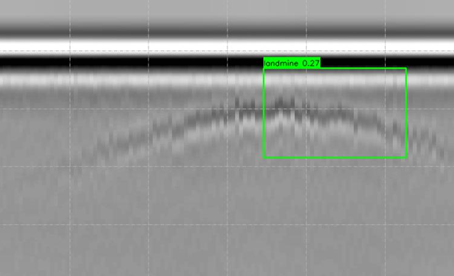
\includegraphics[width=0.32\textwidth]{figs/Rory/sim_bscan_clahe_detection_cropped.png}}
          \hfill
          \adjustbox{valign=c}{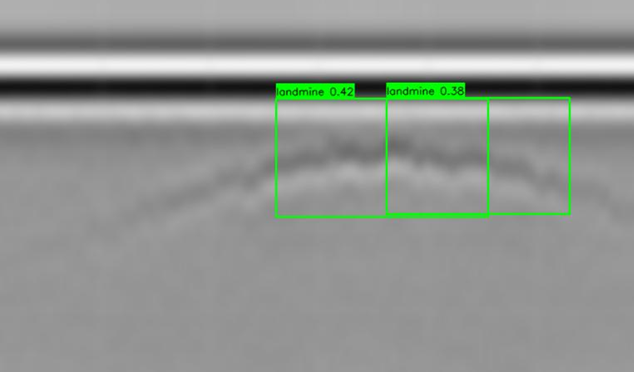
\includegraphics[width=0.32\textwidth]{figs/Rory/sim_bscan_clahe_detection_blur_cropped.png}}
          \hfill
          \adjustbox{valign=c}{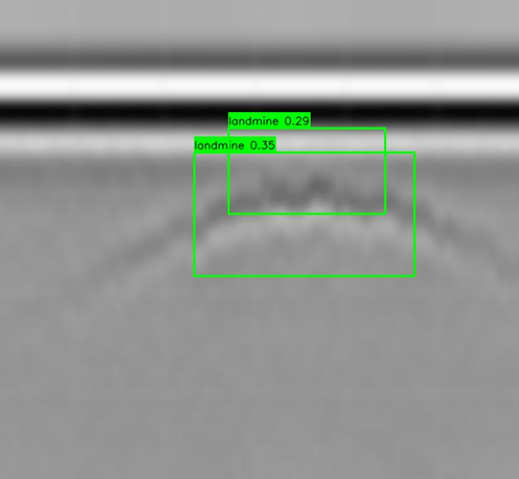
\includegraphics[width=0.32\textwidth]{figs/Rory/sim_bscan_clahe_detection_blur_stretched_cropped.png}}
        
          \caption[Comparison of simulated B-scans under different pre-processing steps]{Comparison of simulated B-scans under different pre-processing steps. 
          \textbf{(a)} Simulated B-scan with CLAHE applied. 
          \textbf{(b)} Simulated B-scan with CLAHE and Gaussian blur applied. 
          \textbf{(c)} Simulated B-scan with CLAHE, Gaussian blur, and a vertical stretch applied. 
          In each case, the bounding boxes from the pre-trained CNN in Section \ref{compvis_implementation} are visible, with the corresponding numerical confidence level.}
          \label{fig:sim_bscan_comparison}
        \end{figure}
        
    
    \subsubsection{CV Results}
    
        The augmented radar data were then fed into the radar CV model (Section \ref{compvis_implementation}) to evaluate the robustness of the model to the physical loss processes described in Section \ref{rory_radar_principles}. Precision and recall metrics were calculated on the augmented dataset, with the results summarised in Table~\ref{tab:cv_results}. The high precision of 91.5\% indicates that the combined approach of GPR and YOLOv11 is well-suited for practical landmine detection. In particular the high precision is achieved with a moderately high recall of 83.3\%, which shows that although the radar computer vision model was trained on a homogenous, 'clean' dataset, it generalised well to a more varied dataset from simulations that directly model noise processes. Therefore, a radar computer vision model trained on a larger dataset of experimentally obtained noisy B-scans should be robust to features not present in the training data, and will generalise well across a range of environmental conditions.

        Overall, this system offers a highly accurate and robust solution for detecting landmines, that can improve as more context specific training data becomes available.

        \begin{table}[htbp]
          \centering
          \caption{Augmented Simulation B-scan Results}
          \label{tab:cv_results}
          \begin{tabular}{@{} l l @{}} 
            \toprule
            \textbf{Metric} & \textbf{Value} \\
            \midrule
            Number of actual landmines & 90 \\
            Number of true positive predictions & 75 \\
            Number of false positive predictions & 7 \\
            Number of false negative predictions &  15\\
            \midrule
            \textbf{Precision} &  \textbf{91.5\%}\\
            \textbf{Recall} & \textbf{83.3\%}\\
            \bottomrule
          \end{tabular}
        \end{table}       
        